\chapter{Basic NEF networks}
When constructing neural models with the NEF, there are certain networks that are often used in multiple places and constitute basic building blocks for larger scale networks.
In the following, I will shortly discuss how to create a differentiator, an integrator, a gated memory buffer based on that integrator, an ensemble applying a threshold to a signal, and how to do multiplication in neurons.

Often it is helpful to use a graphic representation to understand NEF networks.
The graphical primitives used in the network diagrams in this thesis are shown in \cref{fig:tikz-nef}.
Normal ensembles are marked with a circle.
Sometimes the dimensions of a vector will be split across multiple ensembles, called an \emph{ensemble array}, and marked by a stack of circles.
Multiple NEF components that constitute a network not shown in full detail, use rectangles with rounded corners.
Sometimes it is useful to combine decoded representations before transmitting them to the destination neurons in a \emph{pass-through} node.
Such nodes are marked by filled circles.
Note that such pass-through nodes could be replaced with the actual neuron-to-neuron connections and are not biological implausible.
\emph{Rectification ensembles} are useful enough to warrant a special symbol: a rectified linear plot in its circle.
These ensembles are discussed in detail in \cref{sec:thresholding}.
Normal NEF connections are represented by arrows and typically have a synaptic time constant of \SI{5}{\milli\second} which is is in the range of experimentally measured values for AMPA-type glutamate receptors~\parencite{jonas1993,spruston1995-1}.
Linear transforms or functions computed across the connection are denoted along the arrow.
Inhibitory connections bypass the encoders of the target ensemble and use a negative transform to suppress firing in the target ensemble.
Finally, modulatory connections do not influence the representation in an ensemble directly, but the connection weights of another connection.
\begin{figure}
    \hfill
    \begin{tikzpicture}[nef]
        \matrix [row sep=4pt, column sep=4pt] {
            \node [nef,ext] {ext}; & \node [right] {external inputs and outputs}; \\ 
            \node [nef,ens] {$\vc x$}; & \node [right] {ensemble representing $\vc x$}; \\ 
            \node [nef,ea] {$\vc x$}; & \node [right] {ensemble array representing $\vc x$}; \\ 
            \node [nef,net] {net}; & \node [right] {network}; \\ 
            \node [nef,pnode] {}; & \node [right] {pass-through node}; \\
            \node [nef,rect] {}; & \node [right] {rectification ensemble}; \\ 
        };
    \end{tikzpicture}
    \hfill
    \begin{tikzpicture}[nef]
        \matrix [row sep=4pt, column sep=4pt] {
            \draw (-10pt, 0) -- (10pt, 0) [-Latex]; & \node [right] {connection}; \\
            \draw (-10pt, 0) -- node [above] {$\mat T$} (10pt, 0) [-Latex]; & \node [right] {connection with transform $\mat T$}; \\
            \draw (-10pt, 0) -- (10pt, 0) [inhibit]; & \node [right] {inhibitory connection}; \\ 
            \draw (-10pt, 0) -- (10pt, 0) [modulatory]; & \node [right] {modulatory connection}; \\ 
            \node (ens) [nef,ens] {}; \path [nef] (ens) edge [nef,recurrent,-Latex] (ens) ; & \node [right] {recurrent connection}; \\ 
        };
    \end{tikzpicture}
    \hfill
    \caption[Graphical elements in NEF network diagrams]{Graphical elements in NEF network diagrams. See text for further explanation.}\label{fig:tikz-nef}
\end{figure}


\section{Differentiator}
While a perfect differentiator is not physically realizable (it would require infinite gain), it is often sufficient to detect a sudden change in a signal.
For this an approximation can be constructed out of two synaptic low pass filters $\syn_1(t) =  \tau_1^{-1} \exp(t/\tau_1)$ and $\syn_2(t) = \tau_2^{-1} \exp(t/\tau_2)$ with time constants $\tau_1 < \tau_2$ as
\begin{equation}
    \od{\vc x}{t} \approx \vc y(t) = \vc x * h_1 - \vc x * h_2 = \vc x * \del{h_1 - h_2} \text{.}
\end{equation}
\cref{fig:differentiator} shows the impulse and the magnitude response of a differentiator constructed this way.
The attenuation of low frequency is desired as this corresponds to the differentiation.
The attenuation of high-frequencies above the pass-band is undesired, but given appropriate $\tau_1$ and $\tau_2$ unproblematic in a neural network because signals will in general be subject to synaptic filtering of high frequencies.
The implementation of such a differentiator is straight-forward with the NEF (\cref{fig:differentiator-net}) by feeding the same input with two different synaptic time constant into an ensemble.
In this work $\tau_1 = \SI{5}{\milli\second}$ and $\tau_2 = \SI{50}{\milli\second}$ were used which is in the range of experimentally observed neurotransmitter decay constants~\parencite{sah1990-1,moreno-bote2005}.
\begin{figure}
    \centering
    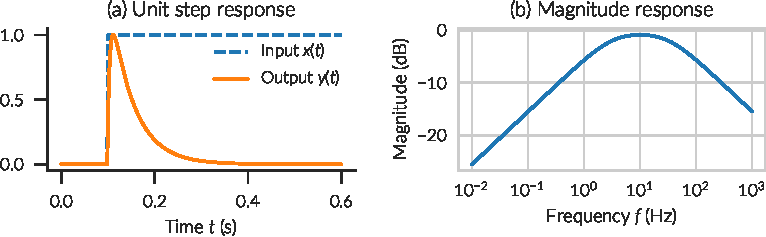
\includegraphics{figures/differentiator}
    \caption[Differentiator]{Differentiator with $\tau_1 = \SI{5}{\milli\second}$ and $\tau_2 = \SI{50}{\milli\second}$. (a) Response of the differentiator to a unit step input. The output has been normalized to the maximum. (b) Magnitude response for sinusoidal inputs with different frequencies.}\label{fig:differentiator}
\end{figure}
\begin{figure}
    \begin{captionbeside}[Implementation of a differentiator with the NEF]{Implementation of a differentiator with the NEF\@. The connection labels state the transform and synaptic time constants with $\tau_1 < \tau_2$.}[i]
        \begin{tikzpicture}[nef]
            \graph {
                x/"$\vc x$" [ens] -> ["$+1, \syntau=\tau_1$", bend left] y/"$\vc y$" [ens];
                x -> ["$-1, \syntau=\tau_2$" below, bend right] y;
            };
        \end{tikzpicture}
    \end{captionbeside}\label{fig:differentiator-net}
\end{figure}


\section{Integrator}
Integrators are important components in many NEF models because they allow to store values over some timespan in neural activity.
An integrator is described by the differential equation
\begin{equation}
    \od{\vc x(t)}{t} = \vc u(t)
\end{equation}
where $\vc u(t)$ is the external input to the integrator.
Applying principle 3 of the NEF tells us that the input has to be scaled by the synaptic time constant $\tausyn$.
Furthermore, a recurrent connection feeding the output of the integrator back to itself is needed (\cref{fig:integrator-net}).
To get a stable representations over a sufficient time window, it is best to use a long time constant like $\tausyn = \SI{0.1}{\second}$ which is the range measured for the NMDA neurotransmitter~\parencite{sah1990-1,moreno-bote2005}.
Due to neural noise and distortion error, the represented value can drift over time (\cref{fig:integrator}).
The distortion in the decoded representation leads to a finite number of fixed points and the represented value will shift to one of the stable fixed points over time.
The neural noise will prevent the representation to stay in an unstable fixed point and can make the representation to move out of the basin of attraction of current stable fixed point.
Adding more neurons to an integrator will make it more stable as the spiking noise will be decreased.
Similarly, a longer recurrent synaptic time constant makes the integrator also more stable.
Increasing the number of represented dimensions will make the integrator less stable because there will be less fixed points.
\begin{figure}
    \begin{captionbeside}{Implementation of an integrator with the NEF}[i]
        \begin{tikzpicture}[nef]
            \path[use as bounding box] (-0.25, -0.6) rectangle (3, 0.6);
            \graph {
                u/"$\vc u$" -> ["$\syntau$" above] x/"$\vc x$" [ens];
                x -> [out=300, in=60, distance=40pt] x;
            };
        \end{tikzpicture}
    \end{captionbeside}\label{fig:integrator-net}
\end{figure}
\begin{figure}
    \centering
    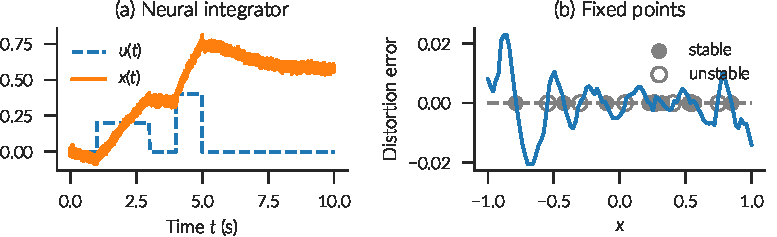
\includegraphics{figures/integrator}
    \caption[Neural integrator]{Neural integrator with 100 neurons and a recurrent synaptic time constant of $\syntau = \SI{100}{\milli\second}$. (a) Example input $u(t)$ and output $x(t)$ of the neural integrator. (b) Distortion error (blue curve) and fixed points. Stable fixed points are marked by filled circles, unstable fixed points by unfilled circles.}\label{fig:integrator}
\end{figure}


\section{Gated memory buffer}
While the integrator enables us to store a value over time, it does not allow for particularly quick updating.
A quicker update can be achieved by adding a difference ensemble (\cref{fig:gated-mem}).
By scaling the difference with a gain factor $g$ the updating speed can be regulated.
However, too large values will lead to oscillations in the integrator.
Note that in this case feeding a null vector to the difference ensemble will clear out the memory instead of keeping the current value.
Thus, the input the integrator needs to be gated.
This can be done by inhibiting the neurons of the difference ensemble to keep the current value in the integrator.
\begin{figure}
    \begin{captionbeside}[Gated memory buffer network]{Gated memory buffer network. The \pop{store} input controls whether the input $\vc u(t)$ is allowed to overwrite the stored value $\vc x(t)$.}[i]
    \begin{tikzpicture}[nef]
        \graph [branch down=40pt] {
            u/"$\vc u$" -> diff/"$\vc u - \vc x$" [ens] -> ["$g \syntau$" above, bend left] x/"$\vc x$" [ens];
            x -> ["-1" below, bend left] diff;
            x -> [out=300, in=60, distance=40pt] x;
            store [ext] -> [inhibit] diff;
        };
    \end{tikzpicture}
\end{captionbeside}\label{fig:gated-mem}
\end{figure}

\section{Thresholding ensembles}\label{sec:thresholding}
Often one needs to apply a threshold to value, i.e.\ implement the function
\begin{equation}
    f(x) = \left\{ \begin{array}{ll}
            0 & x < 0 \\
            x & x \geq 0
        \end{array} \right.
    \text{,}
\end{equation}
or compute the Heaviside step function
\begin{equation}
    \Heavi(x) = \left\{ \begin{array}{ll}
            0 & x < 0 \\
            1 & x \geq 0
        \end{array} \right.
    \text{.}
\end{equation}
Both of these functions are non-differentiable at 0.
The Heaviside function is even discontinuous at that spot.
These properties make it problematic to implement this function with a standard NEF ensemble.
Nevertheless, a good approximations of these functions can be achieved by aligning the neuron's tuning curves according to the shape of these functions.

Instead of choosing encoders randomly as $-1$ and $1$, all encoders are set to $1$ and all intercepts of the neuron tuning curves are chosen from $x \in [0; 1]$.
Choosing the intercept distribution of this interval appropriately can further increase the accuracy.
An exponential distribution that clusters intercepts close to 0 performs best (\cref{fig:thresholding}).
Note that this is even better than setting all intercepts to 0 as this gives more variation in the tuning curves.
The uniform distribution often does not produce intercepts close enough to the threshold value which leads to an increased effective threshold.
\begin{figure}
    \centering
    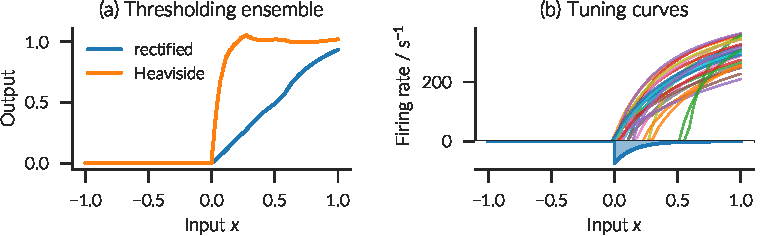
\includegraphics{figures/thresholding}
    \caption[Thresholding ensemble]{Thresholding ensemble with 25 neurons. (a) Decoded rectified and Heaviside output.  (b) Tuning curves in the upper part; probability density function of the exponential intercept distribution with inverted y-axis (i.e.\ probability density increases downward).}\label{fig:thresholding}
\end{figure}


\section{Product}
A product of two scalar numbers $x$ and $y$ could be computed by feeding them into separate dimensions of a two-dimensional ensemble and decoding out the product.
A \SI{37}{\percent} more accurate implementation (with the same number of neurons) is, however, possible~\parencite{gosmann2015-1} by rewriting the product with squares as
\begin{equation}
    xy = \frac{1}{4}\del{x^2 + 2xy + y^2} - \frac{1}{4}\del{x^2 - 2xy + y^2} = \frac{1}{4}\del{x + y}^2 - \frac{1}{4}\del{x - y}^2 \text{.}
\end{equation}
The neural implementation of this equation is straight-forward (\cref{fig:product-net}).
\begin{figure}
    \begin{captionbeside}{Implementation of an accurate product with the NEF}[i]
        \begin{tikzpicture}[nef, x=2cm, y=2cm]
            \graph [no placement] {
                x/"$x$" [at={(0, 1)}] -> sum/"$a$" [ens, at={(1, 1)}] -> ["$a^2/4$"] prod/"" [pnode, at={(2, 0.5)}] -> out/"$xy$" [at={(3, 0.5)}];
                y [at={(0, 0)}] -> ["-1" below] diff/"$b$" [ens, at={(1, 0)}];
                y/"$y$" -> sum;
                x -> diff;
                diff -> ["$b^2/4$" below] prod;
            };
        \end{tikzpicture}
    \end{captionbeside}\label{fig:product-net}
\end{figure}

Multiple scalar product networks can be combined to compute element-wise vector products.
By summing across those element-wise products a dot product can be computed.
Product networks are also used in the computation of circular convolution as binding operation in the Semantic Pointer Architecture (TODO ref section).
